\chapter{Training \& Testing of the
Classifier}
\label{Chapter 4}
Recall from the last chapter that Convolutional Neural Networks (CNNs) are used
in the training of a model for a classifier. Classification is the process
of putting a tag on an image from a set of class labels. This chapter is about the
training of classifier for a dataset of 10000 images with 2000 images of each class.
The step by step process of training a classifier is explained in detail in this chapter. Results obtained from the testing of the classifier by varying certain parameters are recorded and attached
in the latter part of the chapter.
\section{Formation of Dataset}
In deep learning techniques for Classification of images, we have
an example of images which are input to to the system to get a
label from the given classes. This set of images is called dataset.
The dataset is divided into training and dataset by a specific ratio.


In this project we have five different classes of vehciles i.e. Bus, Car, Truck, Motorcycle
and Hiace. There are a total of 10000 images with 2000 images of each 
class. These images are downloaded from Google search results and from already available
datasets and from websites providing licensed free images like Flickr. APIs are available which
can be used along with a simple Python script to download a lot of images.
Using matplotlib in python, we can plot some of the images with the output as
shown in listing \ref{listing:1} and plot is attached in figure
\ref{fig:4.1}.
\begin{listing}[H]
\begin{minted}[bgcolor=bg,
    frame = lines,
    framesep = 2mm]{python}
import matplotlib.pyplot as plt
from matplotlib.image import imread  
path  = './images/'
for i in range(9):
    plt.subplot(330+1+i)
    filename = path + 'image_'+ str(i) + '.jpg'
    image = imread(filename)
    plt.imshow(image)    
    plt.show()
\end{minted}
\caption{Python script to plot some images from each class}
\label{listing:1}
\end{listing}

\begin{figure}[H]
    \centering
    \captionsetup{justification = centering}
    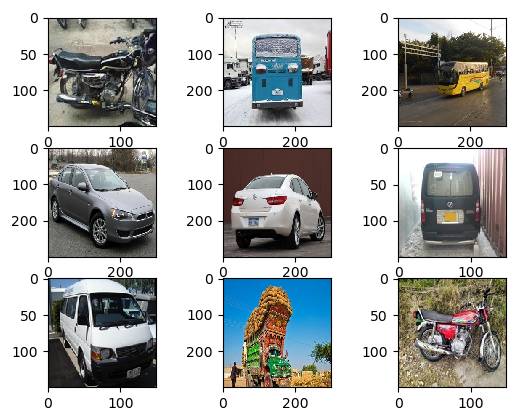
\includegraphics[scale = 0.8]{CHAPTERS/Chapter-4/Images/4.1.png}
    \caption{Plot of some images from each class} 
    \label{fig:4.1}
  \end{figure}

\subsection{Data Augmentation}
Increasing the size of dataset makes the deep learning model to learn and classify images more accurately. This problem of lack of sufficient data can be solved using technique of data augmentation which is used to increase the size of available set of images.
Data augmentation is the process of applying techniques like shifting, flipping, rotating and varying the brightness etc on images to introduce variations among them.

\section{Setting of Workspace for the Project}
\section{Working of Code}
\subsection{Conversion of Images and Labels to Numpy Arrays}
\subsection{Train-Test Division}
\subsection{Conversion to Floats}
\subsection{Subtraction of Mean Pixel}
\subsection{c}at